%%%%%%%%%%%%%%%%%%%%%%%%%%%%%%%%%%%%%%%%%%%%%%%%%%%%%%%%%%%%%%%%%%%%%%%%%%%%%%%
%%% SETUP

\providecommand{\main}{../..}  % for subfiles
\providecommand{\mystyleloc}{../../util}  % for stylesheets
\documentclass[\main/main.tex]{subfiles}

%%%%%%%%%%%%%%%%%%%%%%%%%%%%%%%%%%%%%%%%%%%%%%%%%%%%%%%%%%%%%%%%%%%%%%%%%%%%%%%
%                                 SETTINGS
%%%%%%%%%%%%%%%%%%%%%%%%%%%%%%%%%%%%%%%%%%%%%%%%%%%%%%%%%%%%%%%%%%%%%%%%%%%%%%%
% Implementing Package Settings

\graphicspath{{images/}{\main/images/}}

\title{General Qualifying Exam Solutions: Physics and Fundamentals\\}
\author{{Starkman}, Nathaniel \\%
		\and {Lokken}, Martine \\%
		\and {Ludwig}, Bethany \\%
		\and {Winch}, Harrison%
}
% \date{\today}


%%%%%%%%%%%%%%%%%%%%%%%%%%%%%%%%%%%%%%%%%%%%%%%%%%%%%%%%%%%%%%%%%%%%%%%%%%%%%%%
%                                  DOCUMENT
%%%%%%%%%%%%%%%%%%%%%%%%%%%%%%%%%%%%%%%%%%%%%%%%%%%%%%%%%%%%%%%%%%%%%%%%%%%%%%%

\begin{document}

% -----------------------------------------------------------------------------
%                                  TITLE PAGE
% -----------------------------------------------------------------------------

% \hfill{\textit{Last modified \today}}

\maketitle

% -----------------------------------------------------------------------------
%                                     TOC
% -----------------------------------------------------------------------------

\tableofcontents
\let\tableofcontents\relax


% -----------------------------------------------------------------------------
%                                    INTRO
% -----------------------------------------------------------------------------

\newpage
\section{Introduction} % (fold)
\label{sec:introduction}


	% External Answers

% section introduction (end)


% -----------------------------------------------------------------------------
%                                      Q1
% -----------------------------------------------------------------------------

\section{Q1) Interferometry} % (fold)
\label{sec:q1_interfometer}
\questiontext{A  two-element  interferometer  consists  of  two  telescopes  whose  light is  combined and interfered.  Explain how this might be accomplished in practice, and sketch the response of such an interferometer to a nearby red giant star, as a function of the (projected) separation between the two telescopes.}

    \subsection{Notes}
        $\theta = 2.2 \lambda / D$, D is telescope baseline
        
        the 1.22 in $1.22 \lambda / D$ comes the Rayleigh Criterion for the Fresnel-Kirchoff formula.
        
        Visibility: $V = 2\sqrt{I_1 I_2} / (I_1 + I_2)$
    
    \subsection{Followup}
    \begin{itemize}
        \item Why is LIGO an additive interferometer?
        \item Typical VLBI resolution: milli-arcsec resolution
            https://www.ligo.caltech.edu/page/what-is-interferometer
        \item why is the response function a Bessel function?
        \item why is the response function have minima at multiples of the projected baseline?
    \end{itemize}{}
        

	% External Answers
	\includepdf[pagecommand=\subsection{Campbell Physics Q2},scale=.95,pages=9]{physics_and_fundamentals/Campbell/physics}\includepdf[pagecommand=\large{Campbell Physics Q2},scale=.95,pages=10-14]{physics_and_fundamentals/Campbell/physics}

% section q18_dark_matter_candidates (end)

% -----------------------------------------------------------------------------
%                                      Q2
% -----------------------------------------------------------------------------

\section{Q2) Detector Cooling} % (fold)
\label{sec:q2_detector_cooling}
\questiontext{You don’t usually need to cool down the detectors for short wavelength (e.g., X-ray) observations, but it’s critical to cool down the detectors in long wavelength (e.g.,far-IR) observations.  Why is this, and why is it usually less essential or unnecessary for radio observations?}
    \subsection{Short Summary}
    Today, observations in the range of X-ray to IR are typically made using CCDs. The basic operation is that when a photon hits the detector with energy $h\nu > E_g$, where $E_g$ is the energy gap between the valence and conduction bands of the detector (usually made of silicon), it excites an electron from the valence band to the conduction band and creates an electron-hole pair. However, one of the challenges of CCD imaging is dark current. This occurs when a device is warm: the thermal energy in the detector will free some electrons from the valence band, and they will be collected during readout and be indistinguishable from astronomical signal. For longer-wavelength observations, there is a smaller energy gap which the electrons must cross (thus the detector is sensitive to lower-energy photons). More electrons can be excited to the conduction band by the thermal energy of the device, leading to more dark current at the same temperature. Therefore, cooling is more important for longer-wavelength CCD observations. Radio observations do not use CCDs, they use bolometers to detect incoming electromagnetic waves.
    
    Followup:
    \begin{itemize}
        \item can you make optical bolometers? Yes, I think so
        \item how do radio telescopes work? \href{https://public.nrao.edu/telescopes/radio-telescopes/}{https://public.nrao.edu/telescopes/radio-telescopes/}
    \end{itemize}{}
    
    \begin{figure}
        \centering
        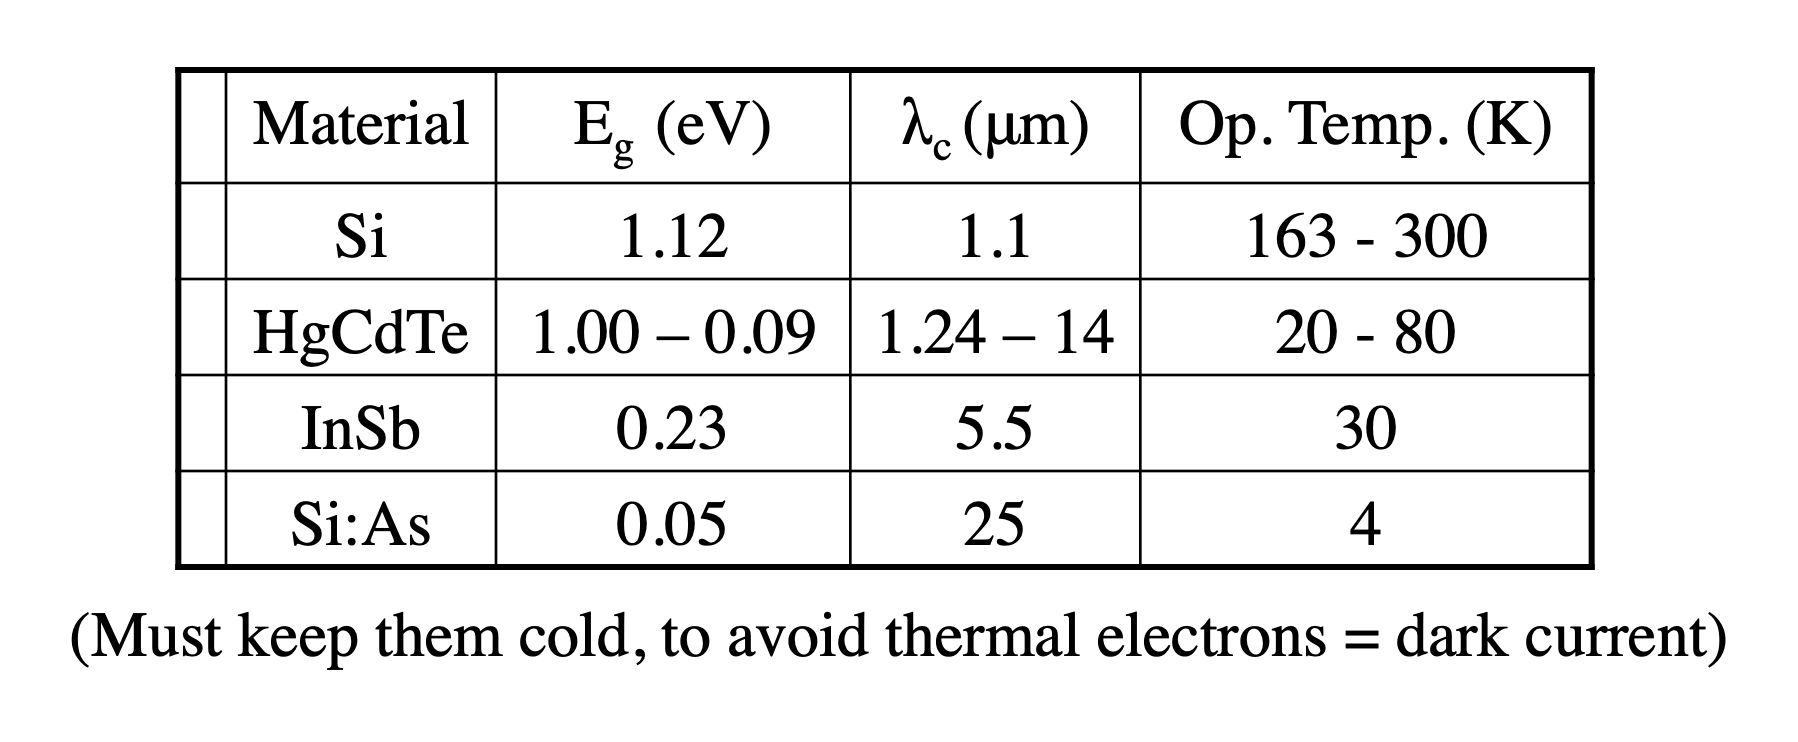
\includegraphics{Answers/images/physics_and_fundamentals/dark_current_materials.png}
        \caption{dark current materials}
        \label{fig:dark_current_materials}
    \end{figure}{}
    
	% External Answers
	\includepdf[pagecommand=\subsection{Campbell Physics Q11},scale=.95,pages=45]{physics_and_fundamentals/Campbell/physics}\includepdf[pagecommand=\large{Campbell Physics Q11},scale=.95,pages=46-53]{physics_and_fundamentals/Campbell/physics}

% section q18_dark_matter_candidates (end)


% -----------------------------------------------------------------------------
%                                      Q3
% -----------------------------------------------------------------------------

\section{Q3) Camera Field of View} % (fold)
\label{sec:q3_camera_field_of_view}
\questiontext{What’s the field of view of a 2K x 2K CCD camera on a 5-m telescope with f/16 focal ratio? The pixel size of the CCD is 20 micron. How does the field of view change if we bring it to a 10-m telescope?}

	increasing the diameter decreases FOV b/c resolution is $\theta = \lambda / D$ and have a tradeoff between resolution and FOV

	% External Answers
	\includepdf[pagecommand=\subsection{Campbell Physics Q14},scale=.95,pages=57]{physics_and_fundamentals/Campbell/physics}

% section q3_camera_field_of_view (end)


% -----------------------------------------------------------------------------
%                                      Q4
% -----------------------------------------------------------------------------


\section{A4) Sidelobes in Diffraction-Limited Detectors} % (fold)
\label{sec:a4_sidelobes_in_diffraction_limited_detectors}

% section a4_sidelobes_in_diffraction_limited_detectors (end)

\questiontext{Explain why diffraction-limited detectors tend to have sidelobes, and how sidelobes can be suppressed in optical and radio observations.}

	% External Answers
	\includepdf[pagecommand=\subsection{Herman Physics Q21},scale=.95,pages=25]{physics_and_fundamentals/Herman/5_Physics}


%%%%%%%%%%%%%%%%%%%%%%%%%%%%%%%%%%%%%%%%%%%%%%%%%%%%%%%%%%%%%%%%%%%%%%%%%%%%%%%

\end{document}
